%
% File eacl2014.tex
%
% Contact g.bouma@rug.nl yannick.parmentier@univ-orleans.fr
%
% Based on the instruction file for ACL 2013 
% which in turns was based on the instruction files for previous 
% ACL and EACL conferences

%% Based on the instruction file for EACL 2006 by Eneko Agirre and Sergi Balari
%% and that of ACL 2008 by Joakim Nivre and Noah Smith

%\documentclass[11pt,letterpaper]{article}
%\usepackage{naaclhlt2015}
%\usepackage{times}
%\usepackage{latexsym}

%%\documentclass[11pt]{article}
%%\usepackage{acl2014}
%%\usepackage{times}
%%\usepackage{latexsym}
%\usepackage{url}
%\usepackage{graphicx}
%\usepackage{color}
%\usepackage{comment}
%\usepackage{times}
%\usepackage{amsmath,amsthm,amssymb}
%\usepackage{multirow}
%\usepackage{url}
%\usepackage{verbatim}
%\usepackage{caption}
%\usepackage{subcaption}
%\usepackage{fixltx2e}
%%\usepackage[options]{natbib}
%\usepackage{float}
%%\usepackage{covington}
%\usepackage{supertabular,booktabs}
%%\usepackage[ruled,vlined,linesnumbered]{algorithm2e}
%\usepackage{enumerate}
%\usepackage{longtable}
%\usepackage{afterpage}
%\usepackage{array}
%%\usepackage{setspace}
%\captionsetup{font={footnotesize}}


%\special{papersize=210mm,297mm} % to avoid having to use "-t a4" with dvips 
%\setlength\titlebox{5cm}  % You can expand the title box if you really have to

%\newcommand{\svmr}{{SVM$^{rank}$}}
%\newcommand{\code}[1]{{\tt {\small #1}}}
%\newcommand{\qn}{{{\bf Q}$^\textbf{{\small N}}$}}
%\newcommand{\ssa}{{{\scriptsize $^{*}$}}}
%\newcommand{\todo}[1]{\textcolor{red}{#1}}

%\title{Spinning Straw into Gold: Using Free Text to Train Monolingual Alignment Models for Non-factoid Question Answering}



%\begin{abstract}
%Monolingual alignment models have been shown to boost the performance of question answering systems by "bridging the lexical chasm" between questions and answers.
%%and associating question words like {\em breakfast} with answer words like {\em pancakes} or {\em cereal}.  %Unfortunately these models have been historically challenging to generate, requiring large and expensive corpora of aligned QA pairs to train.  
%The main limitation of these approaches is that they require semistructured training data in the form of question-answer pairs, which is difficult to obtain in specialized domains or low-resource languages.
%%While these models currently require semistructured training data in the form of question-answer pairs, 
%We propose two inexpensive methods for training alignment models solely using free text, by generating artificial question-answer pairs from discourse structures. Our approach is driven by two representations of discourse: a shallow sequential representation, and a deep one based on Rhetorical Structure Theory. 
%We evaluate the proposed model on two corpora from different genres and domains: one from Yahoo! Answers and one from the biology domain, and two types of non-factoid questions: manner and reason. We show that these alignment models trained directly from discourse structures imposed on free text
%improve performance considerably over an information retrieval baseline and a neural network language model trained on the same data.
%%
%%imposing discourse structure on free text allows high-quality alignment models to be inexpensively trained, and that these models can improve performance up to 49\% (relative) over strong information retrieval and neural network language model baselines. 
%
%\end{abstract}

\chapter{Using Free Text to Train Monolingual Alignment Models for Question Answering \label{chapter:naacl2015}}
%
\section{Introduction}
\vspace{-2mm}

 Question Answering (QA) is a challenging task that draws upon many aspects of NLP.  Unlike search or information retrieval, answers infrequently contain lexical overlap with the question (e.g. {\em What should we eat for breakfast? -- Zoe's Diner has good pancakes}), and require QA models to draw upon more complex methods to bridge this "lexical chasm" \cite{Berger:00}.  These methods range from robust shallow models based on lexical semantics, to deeper, explainably-correct, but much more brittle inference methods based on first order logic.  

Berger et al.~\citeyear{Berger:00} proposed that this "lexical chasm" might be partially bridged by repurposing statistical machine translation (SMT) models for QA. Instead of translating text from one language to another, these monolingual alignment models learn to translate from question to answer\footnote{In practice, alignment for QA is often done from answer to question, as answers tend to be longer and provide more opportunity for association~\cite{Surdeanu:11}.}, learning common associations from question terms such as {\em eat} or {\em breakfast} to answer terms like {\em kitchen, pancakes, or cereal}.

While monolingual alignment models have enjoyed a good deal of recent success in QA (see related work), they have expensive training data requirements,  
requiring a large set of aligned in-domain question-answer pairs for training.
% ms: this footnote dilutes the message: too specific for this discussion.
%\footnote{We have empirically observed that alignment models tend to generalize better between training and test folds when the alignment model is trained on its own fold, further increasing the number of high-quality QA pairs required.}.  
%In most domains these pairs are expensive to generate, and one of the current methodological challenges in QA is locating or building high-quality QA pairs for training and testing. Even large open-domain international evaluations and workshops such as the Text REtrieval Conference (TREC)\footnote{\url{http://trec.nist.gov}} and the Cross Language Evaluation Forum (CLEF),\footnote{\url{http://www.clef-initiative.eu}} are often limited to sets of a few hundred factoid questions, many of which are highly related.  As a result, for open domain QA one often makes use of Community Question Answering (CQA) data from websites such as Yahoo! Answers or Stack Overflow, which offer tens of thousands of questions, but of highly variable quality.  
For low-resource languages or specialized domains like science or biology, often the only option is to enlist a domain expert to generate gold QA pairs --  a process that is both expensive and time consuming.  All of this means that only in rare cases are we accorded the luxury of having enough high-quality QA pairs to properly train an alignment model, and so these models are often underutilized or left struggling for resources. 

Making use of recent advancements in discourse parsing \cite{feng12}, here we address this issue, and investigate whether alignment models for QA can be trained from artificial question-answer pairs generated from discourse structures imposed on free text.
% by imposing structure on inexpensive free text resources instead of using QA pairs.  
We evaluate our methods on two corpora, generating alignment models for an open-domain  community QA task using Gigaword\footnote{LDC catalog number LDC2012T21}, and for a biology-domain QA task using a biology textbook. 

The contributions of this work are:
\begin{enumerate}
\vspace{-3mm}
\item We demonstrate that by exploiting the discourse structure of free text, monolingual alignment models can be trained to surpass the performance of models built from expensive in-domain question-answer pairs. 
\vspace{-3mm}
\item We compare two methods of discourse parsing: a simple sequential model, and a deep model based on Rhetorical Structure Theory (RST)~\cite{mann88}.  We show that the RST-based method captures within and across-sentence alignments and performs better than the sequential model, but the sequential model is an acceptable approximation when a discourse parser is not available.  
\vspace{-3mm}
\item We evaluate the proposed methods on two corpora, including a low-resource domain where training data is expensive (biology).
\vspace{-3mm}
\item We experimentally demonstrate that monolingual alignment models trained using our method considerably outperform state-of-the-art neural network language models in low resource domains.
\end{enumerate}










%the task of question answering (QA) has received considerable attention. However, most of this effort has focused on factoid questions rather than more complex non-factoid (NF) questions, such as manner, reason, or causation questions. Moreover, the vast majority of QA models explore only 
%%similarity models based on 
%local linguistic structures, such as syntactic dependencies or semantic role frames, which are generally restricted to individual sentences. This is problematic for NF QA, where questions are answered 
% not by atomic facts, but 
%by larger cross-sentence conceptual structures that convey the desired answers. Thus, to answer NF questions, one needs a model of what these answer structures look like.
%
%Driven by this observation, our main hypothesis is that the discourse structure of NF answers provides complementary information to state-of-the-art QA models that measure the similarity (either lexical and/or semantic) between question and answer. 
%We propose a novel answer reranking (AR) model that combines lexical semantics (LS) with discourse information, driven by two representations of discourse: a shallow representation centered around discourse markers and surface text information, and a deep one based on the Rhetorical Structure Theory (RST) discourse framework~\cite{mann88}.
%To the best of our knowledge, this work is the first to systematically explore within- and cross-sentence structured discourse features for NF AR. The contributions of this work are:
%\begin{enumerate}
%\vspace{-3mm}
%\item We demonstrate that modeling discourse is greatly beneficial for NF AR for two types of NF questions, manner ({\em ``how"}) and reason ({\em ``why"}), across two large datasets from different genres and domains -- one from the community question-answering (CQA) site of Yahoo! Answers\footnote{\url{http://answers.yahoo.com}}, and one from a biology textbook.  
%%Our results show statistically significant improvements of over 20\%, up to 37\% (relative) on precision at 1 (P@1) when discourse is considered. Crucially, these improvements hold even on top of state-of-the-art LS models~\cite{yih13}.
%Our results show statistically significant improvements of up to 24\% on top of state-of-the-art LS models~\cite{yih13}.
%\vspace{-3mm}
%\item We demonstrate that both shallow and deep discourse representations are useful, and, in general, their combination performs best.
%\vspace{-3mm}
%\item We show that discourse-based QA models using inter-sentence features considerably outperform single-sentence models when answers span multiple sentences.
%\vspace{-3mm}
%\item We demonstrate good domain transfer performance between these corpora, suggesting that answer discourse structures are largely independent of domain, and thus broadly applicable to NF QA. 
%\end{enumerate}
%

%
\section{Related Work}
\label{sec-naacl2015:related work}
%\vspace{-2mm}


Lexical semantic models have shown promise in bridging Berger et al.'s \citeyear{Berger:00} "lexical chasm."  In general, these models can be classified into alignment models \cite{echihabi2003noisy,Soricut:06,Riezler:etal:2007,Surdeanu:11,yao2013} which require structured training data, and language models ~\cite{jansen14,sultan-etal:2014:TACL,yih13}, which operate over free text.  Here, we close this gap in resource availability by developing a method to train an alignment model over free text by making use of discourse structures. 

  
  
%  are focusing here on alignment models, which have shown great promise but also have previously been limited by availability of training data.  We address the need for larger amounts of high quality aligned pairs by investigating methods of imposing structure over free text.... Rhetorical Structure Theory (RST) discourse framework ~\cite{mann88}.

Discourse has been previously applied to QA to help identify answer candidates that contain explanatory text (e.g. Verberne et al. \citeyear{Verberne:2007}).
%conducted an initial analysis of using discourse features derived from Rhetorical Structure Theory (RST)~\cite{mann88} for answer candidate selection, and concluded that while discourse features appeared useful, automated discourse parsing tools were required to test the idea on a larger scale.  
Jansen et al. \citeyear{jansen14} proposed a reranking model that used both shallow and deep discourse features to identify answer structures in large answer collections across different tasks and genres.  Here we use discourse to impose structure on free text to create inexpensive knowledge resources for monolingual alignment. Our work is conceptually complementary to that of Jansen et al. -- where they explored largely unlexicalized discourse structures to identify explanatory text, we use discourse to learn lexicalized models for semantic similarity.

Our work is conceptually closest to that of Hickl et al. \citeyear{hickl2006recognizing}, who created artificially aligned pairs for textual entailment.  Taking advantage of the structure of news articles, wherein the first sentence tends to provide a broad summary of the article's contents, Hickl et al. aligned the first sentence of each article with its headline.  By making use of automated discourse parsing, here we go further and impose alignment structure over an entire text.


%Here, by imposing alignment structure using RST we are able to make use of an entire text instead of being limited to a single sentence.


%Monolingual alignment models have been shown to boost the performance of question answering systems by "bridging the lexical chasm" between questions and answers.


\section{Alignment for question answering}
\label{sec-naacl2015:intro}
%\section{NAACL 2015 Related Work}
%\label{sec:related_work_naacl2015}
%\vspace{-2mm}


For the task of question answering (QA), lexical semantic models have shown promise in bridging \citet{Berger:00}'s "lexical chasm," or the lack of lexical overlap between questions and their answers.  In general, these models can be classified into alignment models \citep{echihabi2003noisy,Soricut:06,Riezler:etal:2007,Surdeanu:11,yao2013}, which are based on the repurposing of machine translation models to operate over aligned question-answer pairs within a single language (and hence require structured training data), and language models ~\citep{jansen14,sultan-etal:2014:TACL,yih13}, which operate over free text.  
This training data requirement of alignment models is their main limitation, as it is difficult to obtain in specialized domains or low-resource languages.
In this Chapter, we focus on closing this gap in resource availability by proposing two inexpensive methods for training alignment models solely using free text by generating artificial question-answer pairs from discourse structures. 
%Our approach is driven by two representations of discourse: a shallow sequential representation, and a deep one based on Rhetorical Structure Theory. 
%Here, we focus on closing this gap in resource availability by developing a method to train an alignment model over free text by making use of discourse structures. 

\subsection{Related Work}
Discourse has been previously applied to QA to help identify answer candidates that contain explanatory text (e.g. \citet{Verberne:2007} \todo{check ref} conducted an initial analysis of using discourse features derived from Rhetorical Structure Theory (RST)~\citep{mann88} for answer candidate selection, and concluded that while discourse features appeared useful, automated discourse parsing tools were required to test the idea on a larger scale.  
\citet{jansen14} proposed a reranking model that used both shallow and deep discourse features to identify answer structures in large answer collections across different tasks and genres.  Here we use discourse to impose structure on free text to create inexpensive knowledge resources for monolingual alignment. Our work is conceptually complementary to that of Jansen et al. -- where they explored largely unlexicalized discourse structures to identify explanatory text, we use discourse to learn lexicalized models for semantic similarity.

%\subsection{Artificial alignments}
Our work is conceptually closest to that of \citet{hickl2006recognizing}, who created artificially aligned pairs for textual entailment.  Taking advantage of the structure of news articles, wherein the first sentence tends to provide a broad summary of the article's contents, Hickl et al. aligned the first sentence of each article with its headline.  By making use of automated discourse parsing, here we go further and impose alignment structure over an entire text.

\subsection{Chapter overview}

The remainder of this Chapter is organized as follows.  In Section \ref{sec-naacl2015:approach} we describe our two approaches to generating artificially aligned text pairs.  Then, in Section \ref{sec-naacl2015:models} we describe our models and model features in more detail.  In Section \ref{sec-naacl2015:experiments} we detail the experimental setup used to evaluate the proposed models on two corpora from different genres and domains: one from Yahoo! Answers and one from the biology domain, and two types of non-factoid questions: manner and reason. In Section \ref{sec-naacl2015:results} we provide the results, showing that these alignment models trained directly from discourse structures imposed on free text
improve performance considerably over an information retrieval baseline and a neural network language model trained on the same data.  Finally, in Section \ref{sec-naacl2015:conclusion} we draw conclusions about our approach.

%
% Example of alignment models
%
%\begin{table}[t!]
%\begin{center}
%\begin{scriptsize}
%\begin{tabular}{l|p{60mm}}
%Passage	& Bob likes apples, which grow in his orchard.  He uses them for cider.  \\
%\hline
%Sequential & Bob likes apples, which grow in his orchard. $\rightarrow$ He uses them for cider. \\
%\hline
%RST & Bob likes apples, $\rightarrow$ which grow in his orchard. \\
% & Bob likes apples, which grow in his orchard. $\rightarrow$ He uses them for cider. \\
%
%
%\end{tabular}
%\end{scriptsize}
%%\vspace{-4mm}
%\caption{{\footnotesize \label{font-table} 
%An example of the alignments produced by the two discourse models.  While the sequential model aligns at sentence granularity capturing only intersentence information, the RST model aligns on finer EDU boundaries, capturing both inter/intrasentence alignments.
%}}
%\vspace{-4mm}
%
%\label{tab:examples}
%\end{center}
%\end{table}


\begin{figure}[t!]
\begin{center}
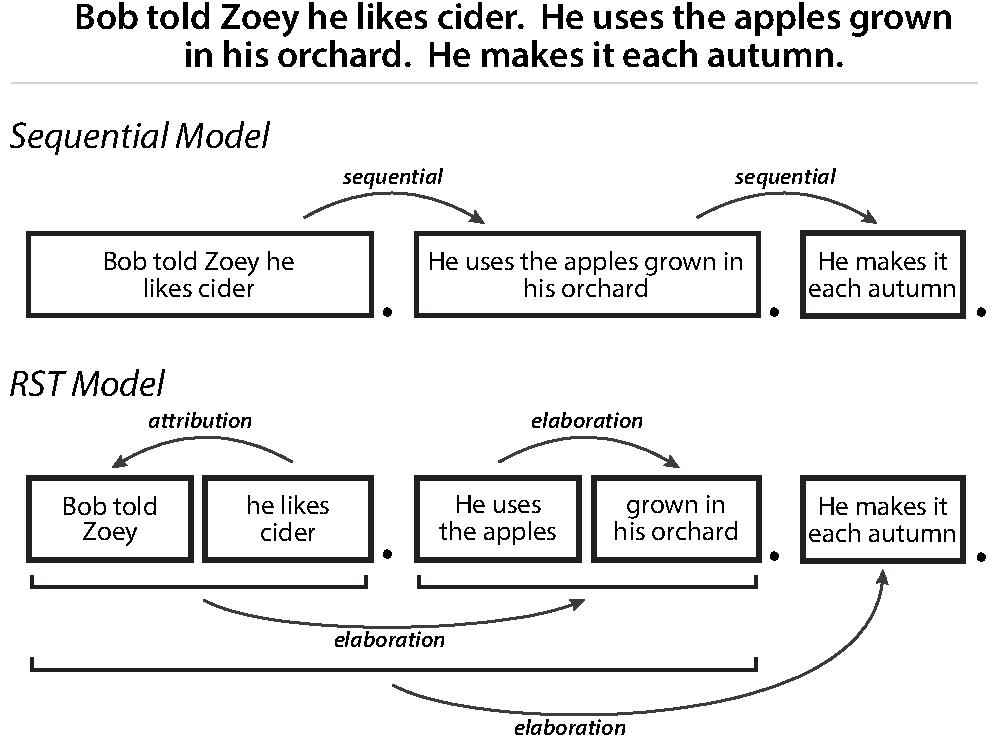
\includegraphics[width=75mm]{mainmatter/naacl2015-alignment/rst2a.pdf}
%space{-2mm}
\caption{{\small An example of the alignments produced by the two discourse models.  The sequential model aligns pairs of consecutive sentences, capturing intersentence associations such as \emph{cider--apples}, and \emph{orchard--autumn}.  The Rhetorical Structure Theory based model generates alignment pairs from participants in all (binary) discourse relations, capturing both intrasentence and intersentence alignments, including 
\emph{apples--orchard, cider--apples}, and \emph{cider--autumn}.}}
\label{fig:examples}
\end{center}
\end{figure}

\section{Approach}
\label{sec-naacl2015:approach}

A written text is not simply a collection of sentences, but rather a flowing narrative where sentences and sentence elements depend on each other for meaning -- a concept known as cohesion~\citep{halliday2014cohesion}.  
Here we examine two methods for generating alignment training data from free text that make use of cohesion: a shallow method that uses only intersentence structures, and a deep method that uses both intrasentence and intersentence structures.
We additionally attempt to separate the contribution of discourse from that of alignment in general by comparing these models against a baseline alignment model which aligns sentences at random.

The first model, the sequential discourse model (SEQ), considers that each sentence continues the narrative  of the previous one, and creates artificial question-answer pairs from all pairs of consecutive sentences.
% ms: no space
%This is similar to a right-attachment baseline in dependency parsing, 
%but operating at sentence granularity rather than word.
Thus, this model takes advantage of intersentence cohesion by aligning the content words\footnote{In pilot experiments, we found that aligning only nouns, verbs, adjectives, and adverbs yielded higher performance.} in each sentence with the content words in the following sentence.  For example, in the passage in Figure \ref{fig:examples}, this model would associate \emph{cider} in the first sentence with \emph{apples} and \emph{orchard} in the second sentence.

The second model uses Rhetorical Structure Theory (RST) to capture discourse cohesion both within and across sentence boundaries.  
We extracted RST discourse structures using an in-house parser~\citep{Surdeanu:15}, which follows the architecture introduced by \citet{hernault10} and \citet{feng12}.
The parser first segments text into elementary discourse units, which may be at sub-sentence granularity, then recursively connects neighboring units with binary discourse relations, such as \emph{Elaboration} or \emph{Contrast}.\footnote{The RST parser performs better on relations which occur more frequently.  We use only relations that occurred at least 1\% of the time.  This amounted to six relations: \emph{elaboration}, \emph{attribution}, \emph{background}, \emph{contrast}, \emph{same-unit}, and \emph{joint}. Using all relations slightly improves performance by 0.3\% P@1.} Our parser differs from previous work with respect to feature generation in that we implement all features that rely on syntax using solely dependency syntax. For example, a crucial feature used by the parser is the dominance relations of \citet{soricut2003}, which capture syntactic dominance between discourse units located in the same sentence. While originally these dominance relations were implemented using constituent syntax, we provide an equivalent implementation that relies on dependency syntax. The main advantage to this approach is speed: the resulting parser performs at least an order of magnitude faster than the parser of \citet{feng12}. 

Importantly, we generate artificial alignment pairs from this imposed structure by aligning the governing text (nucleus) with its dependent text (satellite).\footnote{Pilot experiments showed that this direction of alignment performed better than aligning from satellite to nucleus.} 
 Turning again to the example in Figure \ref{fig:examples}, this RST-based model captures additional alignments that are both intrasentence, e.g., \emph{apples--orchard}, and intersentence, e.g., {\em cider--autumn}. 
% intersentence associations of the sequential baseline, in addition it finds an intrasentence association between \emph{apples} and \emph{orchard}. 

%\todo{The random alignment baseline (RND) was created in a similar fashion to the SEQ model, except that the sentences were randomly shuffled first.  In the open domain this shuffling took place within a document, and in the biology domain it was done across the entire of the textbook.}



%----------------------TABLE FORMAT FROM TACL 2015--------
\begin{table*}[t]{}
        \centering
        \begin{tabular}{p{1cm}p{10cm}}
		\hline        
        \multicolumn{2}{l}{\bf Alignment Models} \\
        \hline
        \multicolumn{2}{l}{Global Alignment Probability:} \\
		  &  p(Q$|$A) according to IBM Model 1 \citep{Brown:93} \\ 
		\\        
        \multicolumn{2}{l}{Jenson-Shannon Distance (JSD) Features:} \\         
         {  } & {Pairwise JSDs were found between the probability distribution of each content word in the question and those in the answer.  The \textbf{mean, minimum, and maximum JSD values} were used as features. Additionally, composite vectors were formed which represented the entire question and the entire answer and the \textbf{overall JSD} between these two vectors was also included as a feature. See \citet{fried2015higher} for additional details.} \\
		\\        
        \hline
		 \multicolumn{2}{l}{\bf Embedding Model} \\
		 \hline
		 \multicolumn{2}{l}{Cosine Similarity Features:} \\        
         {  } & {Similar to \citet{jansen14}, we include as features the {\bf maximum and average pairwise cosine similarity} between question and answer words, as well as the {\bf overall similarity} between the composite question and answer vectors.} \\
        \end{tabular}
        \caption{Feature descriptions for alignment models and the embedding baseline.}
        \label{tab:Features}
	
\end{table*}

%\begin{table*}[h]{}
%
%%\begin{scriptsize}
%
%        \centering
%        %\resizebox{7.9cm}{!}{
%        {
%        %\begin{tabular}{p{1cm}|p{3cm}|l}
%        \begin{tabular}{p{0.3cm}|p{5cm}|p{8cm}}
%        \hspace*{-7pt}  & Feature Group & Feature Descriptions \\
%        \toprule
%        \multirow{10}{*}
%        {\rotatebox[origin=c]{90}{~~~~~~~~~Alignment Models}}
%        & { Global Alignment Probability } & p(Q$|$A) according to IBM Model 1 \cite{Brown:93}\\ 
%        & {} & {}\\
%        & { Jenson-Shannon Distance (JSD) } & {Pairwise JSDs were found between the probability distribution of each content word in the question and those in the answer.  The \textbf{mean, minimum, and maximum JSD values} were used as features. Additionally, composite vectors were formed which represented the entire question and the entire answer and the \textbf{overall JSD} between these two vectors was also included as a feature. See Fried et. al \citeyear{fried2015higher} for additional details.} \\
%        \midrule
%        \multirow{10}{*}
%        {\rotatebox[origin=c]{90}{~~~~~~~~~~~~~~~~~~~~~~~~~~~~~~~~~~RNNLM}}
%        & { Cosine Similarity } & {Similar to Jansen et al.~\citeyear{jansen14}, we include as features the {\bf maximum and average pairwise cosine similarity} between question and answer words, as well as the {\bf overall similarity} between the composite question and answer vectors.} \\
%        \bottomrule
%        \end{tabular}
%        }
%        %}
%
%%\end{scriptsize}
%
%        %\caption{$10$ most important features of each sieve.}
%        \caption{Feature descriptions for alignment models and RNNLM baseline.}
%        \label{tab:Features}
%	\vspace{-6mm}
%
%\end{table*}

%------------------END COPIED TABLE----------------
%space{-1mm}
\section{Models and Features}
\label{sec-naacl2015:models}

We evaluate the contribution of these alignment models using a standard reranking architecture~\citep{jansen14}.
The initial ranking of candidate answers is done using a shallow information retrieval (IR) component.\footnote{We use the same cosine similarity between question and answer lemmas as \citet{jansen14}, weighted using {\em tf.idf}.  Please see \citet{jansen14} for detailed architecture.}  
Then, these answers are reranked using a more expressive model that incorporates alignment features alongside the IR score.  As a learning framework we use \svmr , a Support Vector Machine tailored for ranking.\footnote{ \url{http://www.cs.cornell.edu/people/tj/svm_light/svm_rank.html}}
We compare this alignment-based reranking model against one that uses a state-of-the-art recurrent neural network language model \citep{mikolov10,mikolov13}, which has been successfully applied to QA previously~\citep[e.g.,][]{yih13}.


{\flushleft {\bf Alignment Model:}}  The alignment matrices were generated with IBM Model 1 \citep{Brown:93} using GIZA++~\citep{och03}, and the corresponding models were implemented as per \citet{Surdeanu:11} with a global alignment probability, i.e., the conditional probability of observing a question given an answer.
% ms: the global prob. operates for the whole Q and A!
%question word given an answer word.
\footnote{Within \citet{Surdeanu:11} framework, we lightly tuned the smoothing parameter, $\lambda$, to 0.4 and we redistributed the probability mass for each word such that the probability of a word translating to itself was 0.5.}  
We extend this alignment model with features from \citet{fried2015higher} that treat each (source) word's probability distribution (over destination words) in the alignment matrix as a distributed semantic representation, and make use of the Jensen-Shannon distance (JSD)\footnote{Jensen-Shannon distance is based on Kullback-Liebler divergence but is a distance metric (finite and symmetric).} between these conditional distributions.  A summary of all these features is shown in Table \ref{tab:Features}.% to derive features representing the {\bf minimum, maximum, and average JSDs} between question and answer words, as well as the {\bf overall JSD} between the composite question and answer distributions. 
%Using the Jensen-Shannon distance (JSD) between conditional distributions, content words in each question were compared with the content words in its answers.  Features were made from the maximum, minimum, and average JSDs.  Composite distributions were also created for the entire question and for each entire candidate answer, and the JSD between these composite distributions was used as a feature. 


{\flushleft {\bf Embed:}} We learned word embeddings using the \texttt{word2vec} recurrent neural network language model of \citet{mikolov13}, and include the cosine similarity-based features described in Table \ref{tab:Features}. %Similar to Jansen et al.~\citeyear{jansen14}, we include as features the {\bf maximum and average pairwise cosine similarity} between question and answer words, as well as the {\bf overall similarity} between the composite question and answer vectors. 

%{\flushleft {\bf Hyperparameters}}We used the following very lightly tuned hyperparameters: for \svmr, we used c = 0.1 and for IBM model 1, lambda = 0.4 and self-association of 0.5. \todo{re-write this!! or spread to appropriate places} 

\input{mainmatter/naacl2015-alignment/naacl2015_experiments}
%
%space{-1mm}
\section{Discussion}
\label{sec-naacl2015:discussion}
%space{-2mm}

%
% Alignment performance by part-of-speech association (noun/noun, verb/verb, noun/verb, etc)
%
\begin{comment}
\begin{table}[t!]
\begin{center}
%\begin{scriptsize}
\begin{footnotesize}
\begin{tabular}{llc}
\multicolumn{1}{l}{ } & \multicolumn{1}{l}{ } & \multicolumn{1}{l}{P@1} \\
\multicolumn{1}{l}{ Model/Features } & \multicolumn{1}{l}{P@1} & \multicolumn{1}{l}{Impr.} \\
\cline{2-3}

\hline
\multicolumn{3}{l}{\textit{Yahoo! Answers}} \\ % 185q (sent) ret=1p c=0.1 
\hline
CR Baseline 							& 19.00 					&	  				\\
Full model  							& 29.00 					& +XX\% 			\\
Verb  $\rightarrow$ Verb 				& {\bf XX.XX\ssa}			& {\bf +XX\%}		\\
Verb  $\rightarrow$ Noun 				& {\bf XX.XX\ssa}			& {\bf +XX\%}		\\
Noun  $\rightarrow$ Noun 				& {\bf XX.XX\ssa}			& {\bf +XX\%}		\\

\end{tabular}
%\end{scriptsize}
\end{footnotesize}
%\vspace{-2mm}
\caption{{\footnotesize  Performance of an alignment model trained with only verb$\rightarrow$verb, verb$\rightarrow$noun, or noun$\rightarrow$noun associations on the Y!A corpus.  Performance suggests the effect is primarily driven by XX$\rightarrow$XX associations. 
}}
\label{tab:associationtype}
%\vspace{-4mm}
\end{center}
\end{table}
\end{comment}

The utility of the proposed approach is clear -- by imposing structure over free text,  monolingual alignment can used (with extremely sparse data) to achieve large performance gains in non-factoid QA.  When discourse parsing is possible for the free text in the domain in question, intersentence and intrasentence alignments can be combined to reach maximal performance.  Otherwise, just a straightforward aligning of adjacent sentences can attain a close approximation of those results.  Both of these models far outperform an RNNLM when trained on limited amounts of data.  

In fact, it is notable how quickly we see performance increases from the alignment models in YA.  In both domains, results are increased due to word self-associations (when the same word appears in both the question and the answer), but with YA there also is a slight correlation between answer length and correctness.  The magnitude of the performance increase due to these factors is essentially shown in the results for the smallest sample size, as one document doesn't contain enough data to provide a real alignment contribution.  Taking this into account, the scores still increase quite rapidly for YA.  It could be the case that associations between high frequency verbs drive much of this performance.  If so, then perhaps for the more technical Bio domain, more world-knowledge (encoded in nouns and other parts of speech) is needed,  explaining why we don't see the same immediate performance gain.  To test this, matrices could be made with only verbs, only nouns, or other combinations to determine if one type of association is driving much of the performance and how the domains compare in this respect. 

After a rapid increase, the performance in YA quickly levels off relative to the amount of input for training.~\footnote{Only a fraction of 1 file is used to achieve the maximal performance for the alignment models.  In pilot experiments, including as many as 20 files did not improve performance. }  This may be a result of a decrease in the signal to noise ratio.  Unlike YA, gigaword is within the news domain.  As more and mode documents are added to training, perhaps the model becomes too far biased towards news to continue to increase performance.  If more sophisticated techniques are implemented, such as topic filtering, potentially the performance in this domain could be even higher.  We don't see the same plateau effect with Bio that we do with YA.  Likely this is due to the fact that the in-domain texbook for Bio was much smaller than gigaword.  With more in-domain data we would expect the results for all models to increase, and perhaps the performance curves would resemble those from YA.

\todo{strong close}





%
%space{-1mm}
\section{Discussion}
\label{sec-naacl2015:discussion}
%space{-2mm}

%
% Alignment performance by part-of-speech association (noun/noun, verb/verb, noun/verb, etc)
%
\begin{comment}
\begin{table}[t!]
\begin{center}
%\begin{scriptsize}
\begin{footnotesize}
\begin{tabular}{llc}
\multicolumn{1}{l}{ } & \multicolumn{1}{l}{ } & \multicolumn{1}{l}{P@1} \\
\multicolumn{1}{l}{ Model/Features } & \multicolumn{1}{l}{P@1} & \multicolumn{1}{l}{Impr.} \\
\cline{2-3}

\hline
\multicolumn{3}{l}{\textit{Yahoo! Answers}} \\ % 185q (sent) ret=1p c=0.1 
\hline
CR Baseline 							& 19.00 					&	  				\\
Full model  							& 29.00 					& +XX\% 			\\
Verb  $\rightarrow$ Verb 				& {\bf XX.XX\ssa}			& {\bf +XX\%}		\\
Verb  $\rightarrow$ Noun 				& {\bf XX.XX\ssa}			& {\bf +XX\%}		\\
Noun  $\rightarrow$ Noun 				& {\bf XX.XX\ssa}			& {\bf +XX\%}		\\

\end{tabular}
%\end{scriptsize}
\end{footnotesize}
%\vspace{-2mm}
\caption{{\footnotesize  Performance of an alignment model trained with only verb$\rightarrow$verb, verb$\rightarrow$noun, or noun$\rightarrow$noun associations on the Y!A corpus.  Performance suggests the effect is primarily driven by XX$\rightarrow$XX associations. 
}}
\label{tab:associationtype}
%\vspace{-4mm}
\end{center}
\end{table}
\end{comment}

The utility of the proposed approach is clear -- by imposing structure over free text,  monolingual alignment can used (with extremely sparse data) to achieve large performance gains in non-factoid QA.  When discourse parsing is possible for the free text in the domain in question, intersentence and intrasentence alignments can be combined to reach maximal performance.  Otherwise, just a straightforward aligning of adjacent sentences can attain a close approximation of those results.  Both of these models far outperform an RNNLM when trained on limited amounts of data.  

In fact, it is notable how quickly we see performance increases from the alignment models in YA.  In both domains, results are increased due to word self-associations (when the same word appears in both the question and the answer), but with YA there also is a slight correlation between answer length and correctness.  The magnitude of the performance increase due to these factors is essentially shown in the results for the smallest sample size, as one document doesn't contain enough data to provide a real alignment contribution.  Taking this into account, the scores still increase quite rapidly for YA.  It could be the case that associations between high frequency verbs drive much of this performance.  If so, then perhaps for the more technical Bio domain, more world-knowledge (encoded in nouns and other parts of speech) is needed,  explaining why we don't see the same immediate performance gain.  To test this, matrices could be made with only verbs, only nouns, or other combinations to determine if one type of association is driving much of the performance and how the domains compare in this respect. 

After a rapid increase, the performance in YA quickly levels off relative to the amount of input for training.~\footnote{Only a fraction of 1 file is used to achieve the maximal performance for the alignment models.  In pilot experiments, including as many as 20 files did not improve performance. }  This may be a result of a decrease in the signal to noise ratio.  Unlike YA, gigaword is within the news domain.  As more and mode documents are added to training, perhaps the model becomes too far biased towards news to continue to increase performance.  If more sophisticated techniques are implemented, such as topic filtering, potentially the performance in this domain could be even higher.  We don't see the same plateau effect with Bio that we do with YA.  Likely this is due to the fact that the in-domain texbook for Bio was much smaller than gigaword.  With more in-domain data we would expect the results for all models to increase, and perhaps the performance curves would resemble those from YA.

\todo{strong close}






%space{-2mm}
%\begin{small}
%\section*{Acknowledgments}
%space{-2mm}
%We thank the Allen Institute for AI for funding this work.
%\end{small}

%\bibliographystyle{acl}
%\bibliography{citations} % add your references to citations, then run bibtex

% If you use BibTeX with a bib file named eacl2014.bib, 
% you should add the following two lines:
%\bibliographystyle{acl}
%\bibliography{acl2014}
%\bibliography{refs}
%\bibliography{citations}

